\section{Results \& Discussion - Convection Schemes}
\subsection{Simple Convection}
The simple convective scheme was run for 500 iterations at a time step of 0.02s, Eulers method was used. The number of iterations was selected as at this refereed to an end point where elements showed sufficient "curling up" that the 3d effects of the reactive clustering scheme could be assessed versus the predictive clustering scheme.
\\\\
Figure\ref{fig:SimConvCost} shows the rise in computational cost with increased element count. A trend is clear throughout all data points visually. Further the data points show very high agreement to a quadratic trend with a correlation of $R^2=0.999$. This confirms that the simple unoptimized vortex method does represent an N-Body problem.

\begin{figure}[H]
\centering
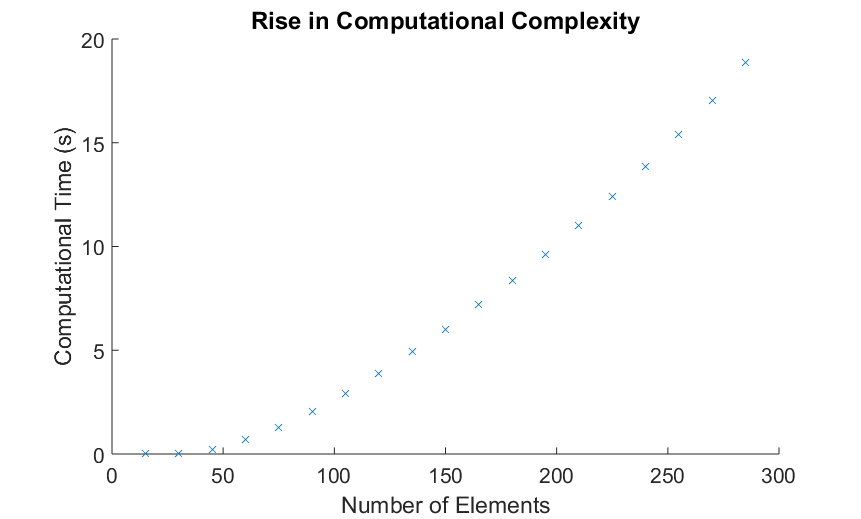
\includegraphics[width=0.8\textwidth]{Figures/SimpleConvCost.png}
\caption{\label{fig:SimConvCost} $ON^2$ Increase in Complexity Demonstrated for an Unoptimized Case}
\end{figure} 

For the maximum grid enlargement, 15 by 30 elements, the positions of all elements were recorded for the final increment so that the results form other schemes could be compared against this. The computational time for the maximum grid size was 21 seconds

\subsubsection{Biasing Schemes}
Figure \ref{fig:RadiusBiasTimes} show the results of increasing the biasing radius on computational time, values were found for the maximum grid size (15 by 30). A constant time of $T=21s$ is plotted on the same axis, this refers to the time taken without the biasing scheme implemented. The radius is dimensionless (the simulation has no inherent units), though the maximum radius encountered for the grid is 25 and the range tested is 0-30, representing 120\% of the maximum radius, hence any trends apparent are captured in the data.
\begin{figure}[H]
\centering
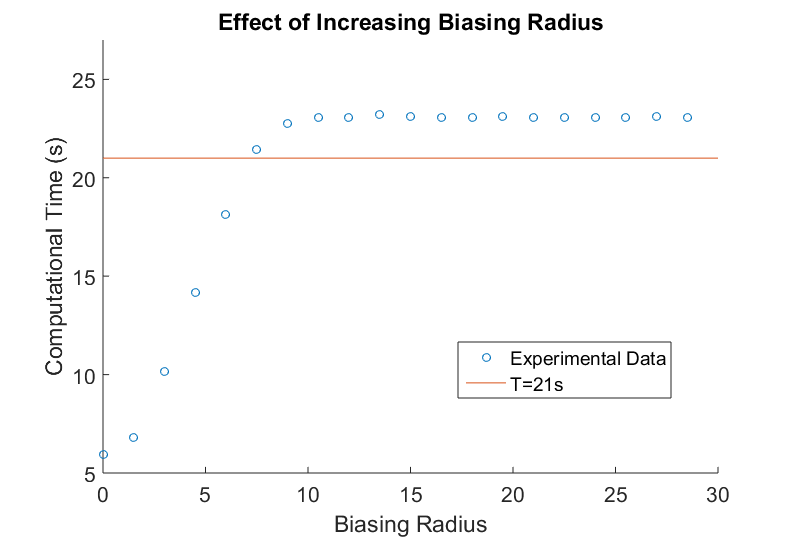
\includegraphics[width=0.8\textwidth]{Figures/RadiusBiasTimes.png}
\caption{\label{fig:RadiusBiasTimes} Increase in computational cost with increased biasing radius}
\end{figure} 

The computational time is initially far lower with the biasing than without, however the computational time increases quickly as the radius increases and the two are equal around $r=7$. Where the computational time is below around 21s represents an optimization, however the computational cost is seen to increase past the cost of implementing no biasing past this. Hence use of a biasing scheme past this point represents a loss in accuracy and decrease in performance. The data appears to settle on a constant value (from around 15 to 30) of around 23, the difference between this and the $T=21s$ represents the additional overhead from implementing the evaluation procedure of the biasing scheme.

\begin{figure}[H]
\centering
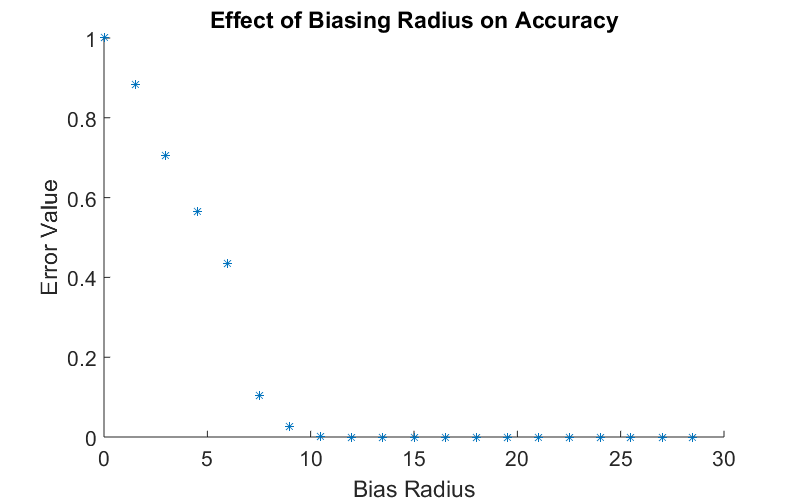
\includegraphics[width=0.8\textwidth]{Figures/RadiusBiasPositionErrors.png}
\caption{\label{fig:RadiusErrors} Effect of increasing biasing radius on accuracy relative to Unoptimized case}
\end{figure} 

Figure \ref{fig:RadiusErrors} shows the effect of increasing the biasing radius on the accuracy (as defined in section) of the simulation. A steep decrease in error is seen immediately as radius is increased. This decrease appears to occur linearly (and shows a correlation of $R^2=0.98$), however this is purely observational and further analysis is required to explain this. The error is seen to decrease to negligible levels before the maximum range is reached. Hence the error is reduced to negligible levels when all elements are not taken into account. 
\\\\
For the range of values of the Bias Radius which represents an optimization (roughly 0-7) the error values seen to range from about 0.9 to 0.1. The lowest of this range, 0.1, still represents an incurred error of about 10\% of the positions of all elements. Hence Biasing methods may be used to optimize a simulation however their effect on accuracy make their use limited for this evaluation criteria.
\\\\
An interesting phenomena was noted during the data processing. The error reduced to zero before the biasing radius had reached the end of its range. An error of exactly zero indicates no difference between the biased case and an unoptimized case. This of course is mathematically impossible, instead this represents an error so small its influence is not captured by the 6 decimal point precision of C\#'s $float$ type variable. This outlines how small of an influence some elements have on others, with their influence being so small it cannot accurately be numerically captured without use of a double precise floating point variable. This indicates there is certainly a good argument for the use of biasing, however more computationally efficient must be employed to see any benefit.
\\\\
\begin{figure}[H]
\centering
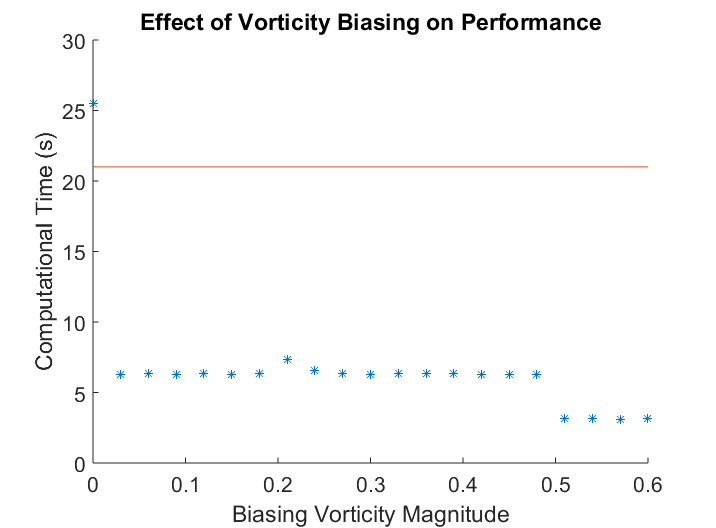
\includegraphics[width=0.8\textwidth]{Figures/VorticityBiasTimes.png}
\caption{\label{fig:VortBiasTimes} Effect on performance of using a vorticity biasing scheme}
\end{figure} 

Figure \ref{fig:VortBiasTimes} shows how the computational time varies with increasing the vorticity bias. The graph is characterised by two regions of constant computational time separated by a discontinuity. This continuity occurs at $|\omega|=0$. The discontinuity is a result of the initial conditions used, the magnitude of the vorticity of elements, which is either $|\omega|=0$ or $0.5$. Hence the first constant section (around $T=5s$) refers to a situation where only non zero vorticity elements are taken into account. Likewise, the situation after the discontinuity (around $T=3s$) represents a situation where no elements are taken into account.
\\\\
At $|\omega|=0$ all elements are taken into account, the computational overhead given by this point is significantly increased over the unoptimized case an is higher than the equivalent case for the radius biasing scheme. This is expected, for the vorticity biasing scheme the magnitude of the vorticity must be found for the evaluation, which represents an increased overhead. Likewise the distance based biasing requires the magnitude of the distance vector to be found, however this value is then used in the Biot-Savart law, so its computation does not result in an increased overhead.
\\\\
Whilst the results may seem promising in figure \ref{fig:VortBiasTimes} it is important to interpret them in the context of the initial conditions used. The initial conditions used were designed to emulate the simulation running in a steady state, so there is no vorticity seeded on the inner rows of elements. However when lift is suddenly generated there is vorticity on these inner elements. Given such initial conditions a continuous trend would be exhibited for the computational times and in retrospect may have been more appropriate. However from the current data it can be concluded that the evaluation procedure for a vorticity based biasing method represents a larger computational overhead than distance biasing.
\\\\
Vorticity based biasing schemes may also become inappropriate in situations where low vorticity elements become close to each other and thus become very influential. This, combined with the increased overhead compared to distancing biasing makes them inappropriate, in their current form, for use in the simulation.

\subsection{Predictive Fixed Cluster Scale}
Figure \ref{fig:FixedClusterTimes} shows the computational times of the fixed size cluster scheme for the same conditions as previously tested. The data from the unoptimized case is included for comparison. At a grid spacing of $15x20$ (referring to 300 elements) the computation time is seen to roughly double for a cluster size of $1x1$ compared to the unoptimized case. This represents the increased overhead from the addition of calculating cluster groupings and cycling through individual elements In an inefficient way. However, this should become more efficient as the the cluster size increases. 
\\\\
This is definitely exhibited in the data, the data points referring to cluster sizes of $3x3$ and $5x5$ are significantly lower than the $1x1$ cluster, being around a fourth at 300 elements. They are also lower than the unoptimized case notably. At a grid size of 225 (the only number of elements where data exist for all data sets) the two clustering schemes have times of $8.1s$ and $4.6s$ for the $3x3$ and $5x5$ respectively. Compared to the time form the unoptimized case for this element count of $11.6s$ an optimization it terms of performance has definitely been achieved.

\begin{figure}[H]
\centering
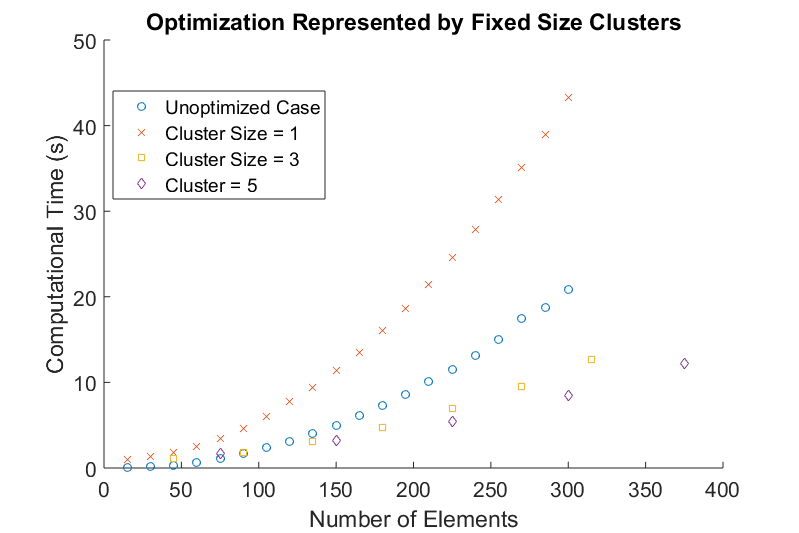
\includegraphics[width=0.9\textwidth]{Figures/FixedClusterSizeTimes.png}
\caption{\label{fig:FixedClusterTimes} Relationship between cluster size and computational time (this graph is made with data with the if statement still in, fix for final version!)}
\end{figure} 

To determine whether this optimization is useful its effect on accuracy must be considered. The errors for the for the three different cluster sizes are shown in table \ref{tab:FixedClusterErrors}. The error for a cluster size of $1x1$ was determined in order to confirm that the it gave results equal to that of the unoptimized case. As the error is zero this has been confirmed and thus the implementation of the clustering scheme is giving the expected mathematical results
\\\\

\begin{table}[H]
\centering
\label{tab:FixedClusterErrors}
\begin{tabular}{llllll}
\multicolumn{1}{l|}{Cluster Size} & 1x1 & 3x3   & 5x5 \\ \hline
\multicolumn{1}{l|}{Error}        & 0   & 0.088 & 0.110 
\end{tabular}
\caption{Calculated Errors for a 15x15 grid for three different cluster sizes.}
\end{table}

The errors for the $3x3$ and $5x5$ cluster sizes are remarkable, an optimization has been achieved in terms of performance and the trade off for accuracy is notably improved over the biasing methods. Further analysis of the element positions visually revealed that the errors were largely caused by elements on cluster boundaries. Figure \ref{fig:FixedClusterPositions} shows the position of the elements predicted by the unoptimized scheme and cluster sizes of $3x3$ and $5x5$ for 500 iterations. 

\begin{figure}[H]
\centering
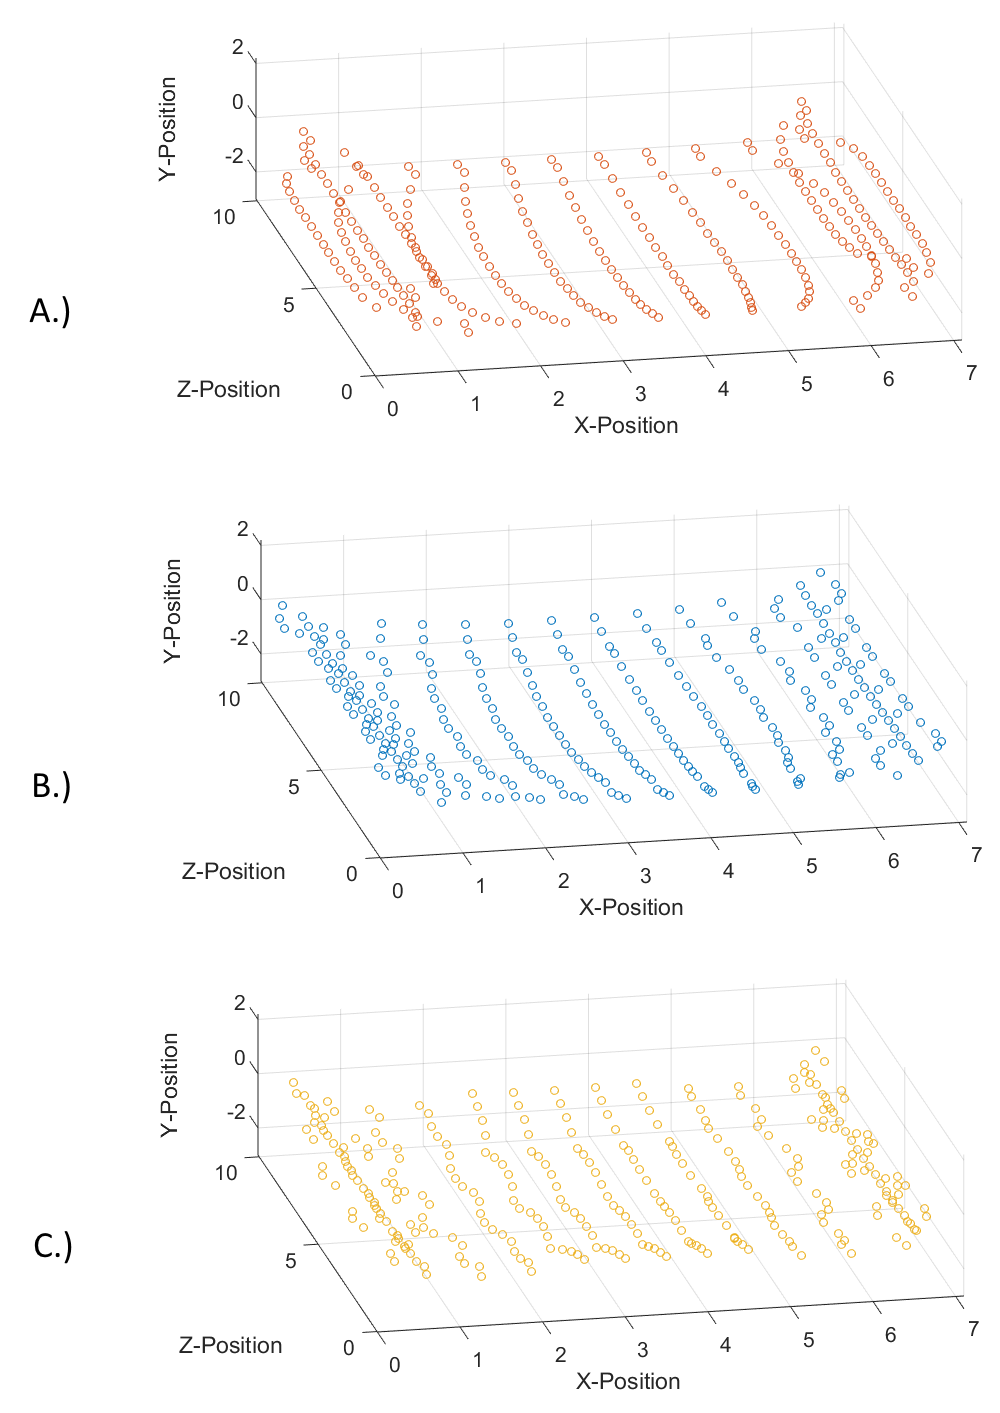
\includegraphics[width=0.7\textwidth]{Figures/FixedClusterImpression.png}
\caption{\label{fig:FixedClusterPositions} Final positions of elements for the unoptimized case (A), cluster size of $3x3$ (B) and $5x5$ (C)}
\end{figure} 

It can be be seen qualitatively that the jump from no clustering to a $3x3$ cluster imposes inaccuracies. This can be seen exhibited in the curvature of the central rows of elements running along the z direction. The difference is notable between the unoptimized case and the $3x3$ cluster sizing. However the for the $5x5$ cluster size large deviations from the unoptimized case are seen and the cluster boundaries are clearly visible along the central elements spanning across the Z direction. This is likely caused by elements inside of a cluster being on that clusters boundary. This would cause the most influential elements to that element, the neighbouring elements, being treated as a mix of elements (neighbours in its own cluster) and clusters (neighbours in a neighbouring cluster).Hence this problem could be resolved via treating the the neighbouring clusters as individual elements as well.
\\\\
The edges of the data points, where elements have vorticity, are seen to roll up. There is significant deviation between the unoptimized case the and the clustered data sets. This is likely due to the vorticity being approximated to act at a different location for each case. The use of a weighted average approach to determining cluster position would likely reduce this error.
\subsection{Dynamic Cluster Size}
Figure \ref{fig:DynamicClusterTimes} shows the computational times of the dynamic cluster size scheme on the same axes as the unoptimized case. A remarkable decrease in computational time is shown represented by the dynamic cluster scheme compared to unoptimized case. Given a computational time of $5.5s$ the dynamic clustering scheme processed 1024 elements whilst the unoptimized case handled 139 elements in $4.9s$. Hence it is obvious that the dynamic cluster scheme represents a definite increase in performance.

\begin{figure}[H]
\centering
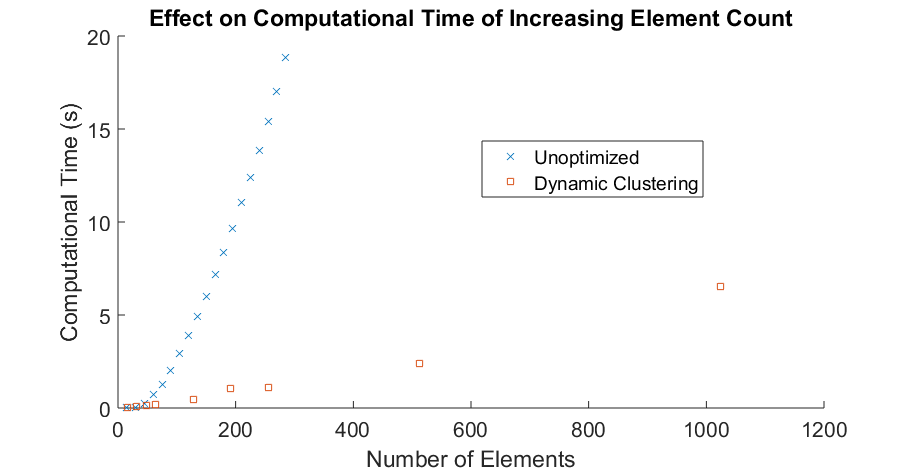
\includegraphics[width=1.0\textwidth]{Figures/DynamicClusterSize.png}
\caption{\label{fig:DynamicClusterTimes} Increase in computational time given increased element count for the unoptimized case and dynamic cluster scaling}
\end{figure} 

The performance increase from the dynamic clustering scheme is larger than that of the fixed sized cluster scheme significantly. Further the $ON^2$ relation appears to have been reduced as well.Whether the predicted relation of $ONlog(N)$ has been exhibited is hard to asses however a least squares regression line of the data points shows a correlation coefficient of 0.99. To determine 
\\\\
The accuracy for the dynamic clustering scheme was 0.051 after 500 iterations with a grid size of 16x20. This is lower than both fixed cluster sizes and the computational time was significantly lower. 
